\documentclass{standalone}
\usepackage{tikz}
\usepackage{mathrsfs}
\usetikzlibrary{positioning, shapes.geometric, arrows}
\usepackage[T1]{fontenc}
\renewcommand*\familydefault{\ttdefault} %% Only if the base font of the document is to be typewriter style
\begin{document}
	 \setbeamercovered{invisible}
	 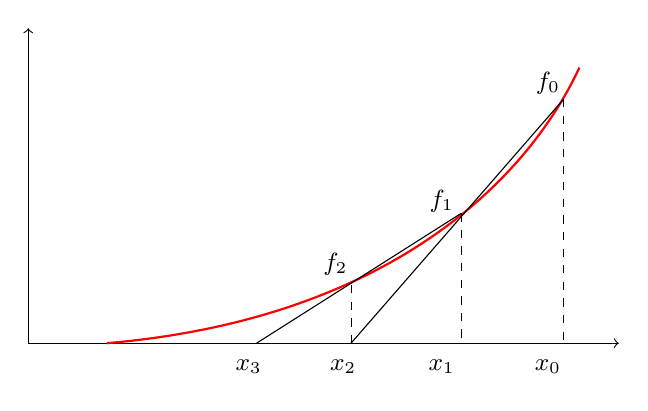
\begin{tikzpicture}[font=\small]
		\draw [->] (0,0) -- (7.5,0);
		\draw [->] (0,0) -- (0,4);
		\draw [red, thick](7,3.5) .. controls (6.3,2) and (4.5,0.3) .. (1,0);
		\draw [dashed] (6.8,3.1) -- (6.8,0);
		\draw (6.6,-0.3) node {$x_{0}$};
		\draw (6.6, 3.3) node {$f_{0}$};
		\draw [dashed] (5.5,1.65) -- (5.5,0);
		\draw (5.25,-0.3) node {$x_{1}$};
		\draw (5.25, 1.8) node {$f_{1}$};
		\draw (6.8,3.1) -- (4.1,0);\pause
		\draw (4,-0.3) node {$x_{2}$};
		\draw [dashed] (4.1,0) -- (4.1,0.8);
		\draw (3.9, 1) node {$f_{2}$};\pause
		\draw (5.5,1.65) -- (2.9,0);
		\draw (2.8,-0.3) node {$x_{3}$};
	\end{tikzpicture}
\end{document}